% model comparison

\par In order to select the best set of features for our $X$ matrix, and also 
compare the use of a single condition feature vs each of the 3 different types
of conditions as 3 seperate features we decided to utilize model comparison, 
specificially AIC,BIC, and Adjusted $R^2$ metrics. Using small expressive
subset of the subjects ($002$,$003$, and $014$) we abused the metric's by
averaging across all voxels and people.  We visualized values in the Figures
\ref{fig:AIC},\ref{fig:BIC}, and \ref{fig:adjR2}, where the x axis follows the 
following structure in Table \ref{tab:plot}.

\par From these plots, you can observe that we don't gain my from adding
the conditions seperated, and from the BIC, we decided that the fourier
features didn't add enough benefit to justify the increase of features, so we'll
be using the model that includes a single HRF for all the conditions, a linear
drift feature, and the first 6 principle components.

\begin{table}
\centering
	\begin{tabular}{l ||  l   |  l  |   l    | l  | l  |  l}
X value & 1 &        2       &             3       &     4         &        5        &         6       \\
	 \hline
	 & HRF &   HRF       &  HRF            & HRF         &  HRF        & HRF  \\
	 &        &   + DRIFT &  + DRIFT      & + DRIFT  &  + DRIFT   & + DRIFT  \\
	 &        &                 &  + FOURIER &  + PCA 4 &  + PCA 6   & + FOURIER \\
	 &        &                 &                      &                &                   & +  PCA 6 \\
	

	\end{tabular}
\caption{Explaining Plot X values}
\label{tab:plot}
\end{table}


%\begin{table}
%
%\begin{minipage}[b]{1\linewidth}
%	\centering
%	\scriptsize{\begin{tabular}{l ||   l  |  l  | l  | l  |l   |  l}
%	 & HRF &   HRF     &  HRF       & HRF      &  HRF       & HRF  \\
%	 &     &   + DRIFT &  + DRIFT   & + DRIFT  &  + DRIFT   & + DRIFT  \\
%	 &     &           &  + FOURIER &  + PCA 4 &  + PCA 6   & + FOURIER \\
%	 &     &           &            &          &            & +  PCA 6 \\
%	\hline
%	All conditions together   &  589.313 &  503.388 &  452.366 & 337.296 & 288.452 &   266.126 \\
%	All conditions seperately & 587.824 &  501.184 &  449.337 &   331.995 & 286.85 &   264.756 \\
%	\end{tabular}}
%	\label{tab:AIC}
%	\center{\caption{AIC}}
%\end{minipage}	
%
%\begin{minipage}[b]{1\linewidth}
%	\centering
%	\scriptsize{\begin{tabular}{l ||   l  |  l  | l  | l  |l   |  l}
%	 & HRF &   HRF     &  HRF       & HRF      &  HRF       & HRF  \\
%	 &     &   + DRIFT &  + DRIFT   & + DRIFT  &  + DRIFT   & + DRIFT  \\
%	 &     &           &  + FOURIER &  + PCA 4 &  + PCA 6   & + FOURIER \\
%	 &     &           &            &          &            & +  PCA 6 \\
%	\hline
%	All conditions together    &  596.409 &  514.032 &  477.202 &    365.68 &316.835&  308.702\\
%	All conditions seperately & 602.016 &  518.924 &  481.269  360.379 & &  322.33 & 314.427 \\
%	\end{tabular}}
%	\label{tab:BIC}
%	\caption{BIC}
%\end{minipage}	
%
%
%\begin{minipage}[b]{1\linewidth}
%	\centering
%	\scriptsize{\begin{tabular}{l ||   l  |  l  | l  | l  |l   |  l}
%	 & HRF &   HRF     &  HRF       & HRF      &  HRF       & HRF  \\
%	 &     &   + DRIFT &  + DRIFT   & + DRIFT  &  + DRIFT   & + DRIFT  \\
%	 &     &           &  + FOURIER &  + PCA 4 &  + PCA 6   & + FOURIER \\
%	 &     &           &            &          &            & +  PCA 6 \\
%	\hline
%	All conditions together    & 0.007  &  0.198  &  0.323  &  0.527   &  0.596  & 0.631 \\
%	All conditions seperately & 0.02   &  0.211  &  0.337  &    0.536  & 0.601  & 0.635\\
%	\end{tabular}}
%	\label{tab:adjR2}
%	\caption{Adjusted $R^2$}
%\end{minipage}
%
%\end{table}



\begin{figure}
\centering
	\begin{minipage}[b]{0.33\linewidth}
		\centering
		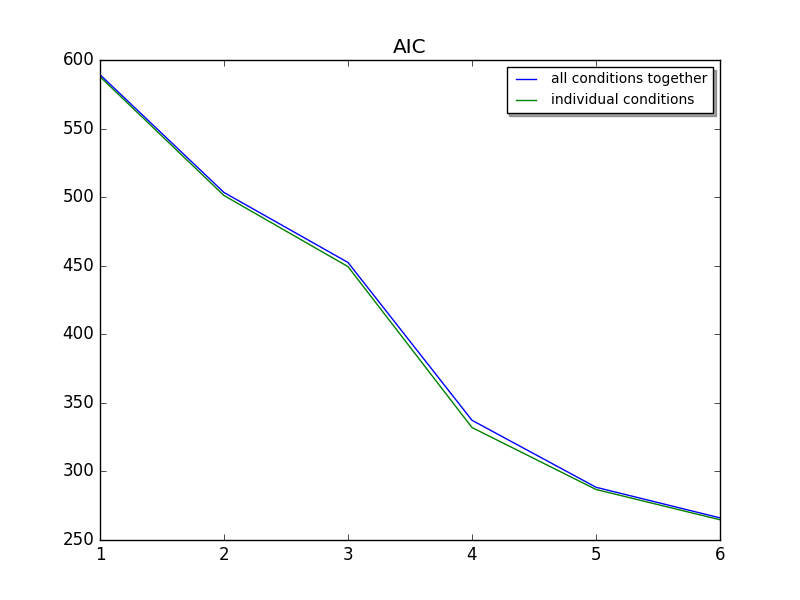
\includegraphics[width=.8\linewidth]{images/aic_better}  

		\caption{AIC}
		\label{fig:AIC}

	\end{minipage}
	\quad
	\begin{minipage}[b]{0.33\linewidth}
		\centering
		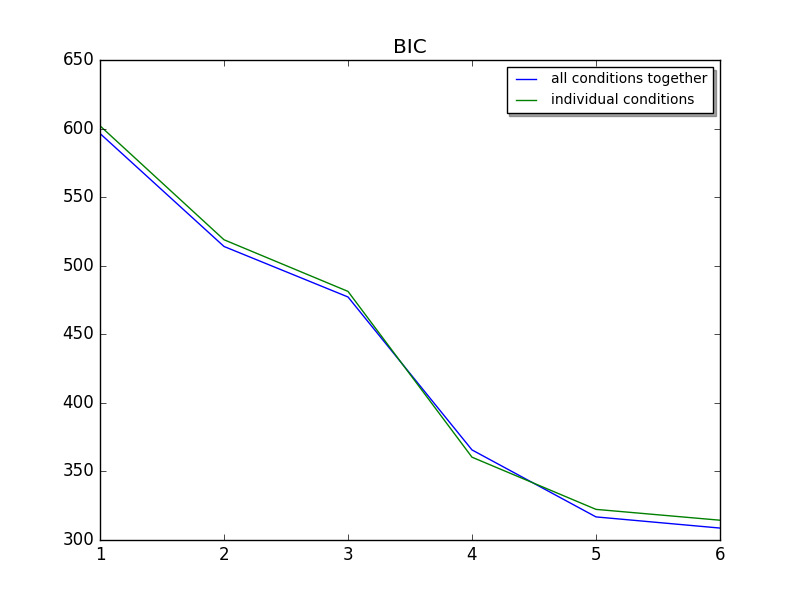
\includegraphics[width=.8\linewidth]{images/bic_better}  
		\caption{BIC}
		\label{fig:BIC}

	\end{minipage}
		
	\begin{minipage}[b]{0.33\linewidth}
		\centering
		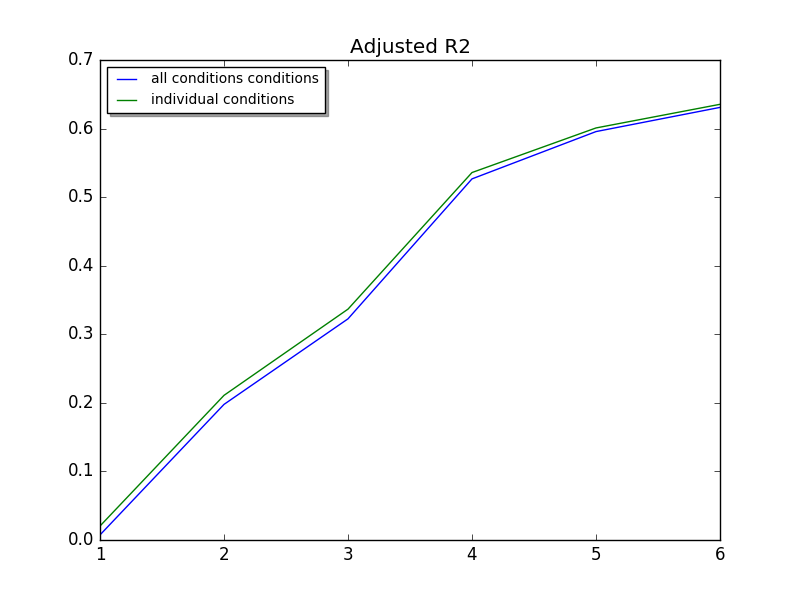
\includegraphics[width=.8\linewidth]{images/adjr2_better}  
		\caption{Adjusted $R^2$}
		\label{fig:adjr2}

	\end{minipage}

\end{figure}

	
	